\documentclass[11pt,a4paper]{article}
\usepackage[margin=25mm]{geometry}
\usepackage[T1]{fontenc}
\usepackage[utf8]{inputenc}
\usepackage{lmodern,amsmath,amssymb,graphicx,booktabs,microtype}
\usepackage[hidelinks]{hyperref}
\usepackage[backend=biber,style=numeric,sorting=none]{biblatex}
\addbibresource{../latex/referencias/referencias.bib}
\title{Separating compression, likelihood approximation and dispersive response errors in simulated pulsar timing arrays}
\author{Gráviton de Souza\thanks{User-requested provisional pseudonym. Authorship and affiliations must be finalized before submission.}}
\date{Draft for review; September 2026}
\begin{document}
\maketitle
\begin{abstract}
Inference from stochastic backgrounds involves distinct choices of frequency compression and likelihood approximation. We study their separation in a periodic Fourier experiment for a dispersive tensor background in pulsar timing arrays. The comparison retains complex coefficients, constructs quadratic estimators, compresses their means and covariances consistently, and changes the response while holding the compressed observation fixed. An exactly Gaussian control isolates information loss from the non-Gaussian distribution of the physical quadratic estimators. A final campaign uses two coupled configurations, with 12 pulsars and four frequencies or 16 pulsars and eight frequencies, and 596 realizations per configuration, yielding 10728 conditional posterior analyses. Sky directions are taken from public MeerKAT metadata; all distances, signals and noise are synthetic. Interval-sensitive calibration tests retain numerically unresolved targets. Separate Holm families contain 42 correctly specified and 84 approximate-model tests. They yield respectively zero and one persistent rejection, with three and one indeterminate decisions. For 500 prior draws, the paired mean information loss from Gaussian compression is $0.06211\pm0.00477$ and $0.10631\pm0.00695$ nat in the two configurations, where uncertainties are Monte Carlo standard errors. These results establish conditional information loss and a specific likelihood-approximation failure, rather than a universal validity criterion for a frozen response. No observational graviton-mass constraint is inferred.
\end{abstract}

\section{Introduction}
A dispersive gravitational-wave response depends on both frequency and pulsar geometry. Replacing it by a response at one reference frequency is therefore a model approximation whose inferential consequences need to be tested. However, comparisons may simultaneously change the retained data, the likelihood family and the response itself. A difference between resulting mass posteriors cannot then be attributed uniquely to frequency compression.

Full-covariance, multifrequency graviton-mass forecasts are already available, including PTA--astrometry estimators \cite{han2026}. The breakdown of Gaussian approximations to stochastic-background likelihoods and its connection to compression have also been studied \cite{franciolini2025}. We do not claim either full covariance or Gaussian-approximation diagnostics as a new principle. Our proposed contribution is a reproducible comparison contract for dispersive PTA responses, with matched observations and explicit propagation of unresolved numerical decisions. Priority for this combination remains a matter for scholarly review.

The numerical experiment is deliberately conditional. It does not fit pulse arrival times, infer a timing model, or marginalize all noise parameters. This restriction supplies a known generator and isolates approximation effects; it limits any interpretation as an observational forecast. We present the completed population extension as the main example and explain how it relates to the broader validation programme archived with the companion dissertation.

\section{Experiment and comparison contract}
\subsection{Periodic data and dispersion}
For positive Fourier frequencies $f_k=k/T$, let $q_k$ be a proper complex Gaussian vector,
\begin{equation}
 q_k\sim\mathcal{CN}(0,C_k(u)),\qquad
 C_k=P_{\rm GW}(f_k)\Gamma_k(u)+N_k,\qquad
 u=f_gT\in[0,1].
\end{equation}
Frequencies are independent by definition of the periodic experiment. The dispersion variable is $\beta_k=\sqrt{1-(u/k)^2}$ and the mass conversion is $m_gc^2=hu/T$. The prior is uniform in $u$. This finite support is a modeling choice, not an empirical bound. The response includes Earth and pulsar terms, evaluated with harmonic expansions and independent sky-integration checks, following the dispersive PTA setting of Refs.~\cite{liang2021,cordes2025}. With transverse tensor polarizations of norm two, the convention is
\begin{align}
 R_a^A&=\frac{p_a^ip_a^je^A_{ij}}{2(1+\beta\widehat\Omega\cdot p_a)}
 [1-e^{-iy_a(1+\beta\widehat\Omega\cdot p_a)}],\\
 \Gamma_{ab}&=\frac{3}{8\pi}\int d\Omega\sum_{A=+,\times}R_a^A R_b^{A*}.
\end{align}
Removable denominator singularities are evaluated by a sinc representation. The pulsar-term dependence is retained, rather than taking an infinite-distance limit throughout.

For a real quadratic statistic $X_i=q^\dagger H_iq$ with Hermitian $H_i$, the proper-complex Gaussian generator gives
\begin{equation}
 \mu_i=\operatorname{tr}(H_iC),\qquad
 \Sigma_{ij}=\operatorname{Re}\operatorname{tr}(H_iCH_jC).
\end{equation}
In each frequency there are ten estimators: real and imaginary cross powers averaged uniformly in four equal-count bins of ordered pair cosines, plus two auto-power bins sorted by nominal timing precision. Bin definitions use only fixed geometry and nominal errors. Thus A contains 40 or 80 real coordinates and B contains ten. Frequency compression is $B_i=K^{-1}\sum_k X_{ki}$ on the fixed, scaled coordinates described below; it is not fitted to the realization.

These moments do not make the joint distribution of $X$ Gaussian. We define A0 as the complex-coefficient likelihood, and A as a normal likelihood for the quadratic estimators using these moments. B applies a fixed linear compression $W$ to A, with $\mu_B=W\mu_A$ and $\Sigma_B=W\Sigma_AW^{\mathsf T}$.

The response controls use the same observed B. In $C_\beta$, the relative propagation-speed argument of the response is set to $\beta_1(u)=\sqrt{1-u^2}$ in every channel while the physical channel-dependent phase scale $y_k=2\pi f_kL/c$ is retained. In $C_{\rm full}$, the entire response is evaluated at its first-channel value $\Gamma(\beta_1(u),y_1)$ for the same mass. Physical spectral and noise factors remain unchanged. These controls are specified approximations, not interchangeable definitions of every possible effective-frequency scheme. Means and covariances are recomputed for each response. Both controls retain mass dependence. The normalized densities used for A0 and for a real normal vector $x$ are
\begin{align}
 \log p(q\mid u)&=-\sum_k[n_p\log\pi+\log\det C_k+q_k^\dagger C_k^{-1}q_k],\\
 \log p(x\mid u)&=-\tfrac12[d\log(2\pi)+\log\det\Sigma+
 (x-\mu)^{\mathsf T}\Sigma^{-1}(x-\mu)].
\end{align}
For A the latter expression sums independent frequency blocks; for B and C it uses the compressed covariance. We do not compare absolute evidences across different observed data spaces.

\subsection{Exactly Gaussian control}
To separate compression from the quadratic distribution, write $C=LL^\dagger$ and $A_i=L^\dagger H_iL$. Let $Z$ be a random Hermitian matrix with independent standard normal diagonal entries and off-diagonal entries $(x+iy)/\sqrt2$, where $x,y$ are independent standard normals. Define
\begin{equation}
 Y_i=\operatorname{tr}(H_iC)+\operatorname{tr}(A_iZ).
\end{equation}
Then $Y$ is jointly real Gaussian with the same $\mu$ and $\Sigma$ as $X$. The construction also preserves the cross-covariance between the two pulsar configurations by embedding both sets of estimator matrices in the same 16-pulsar space. The physical CN and Gaussian G experiments use independent latent banks conditional on the same true mass. Within each bank, the prescribed comparisons share observations.

\subsection{Population design}
We compare P12K4 and P16K8 at $T=4.5$ years. Sixteen sky directions are selected deterministically from public MeerKAT timing-model metadata, using a greedy maximum-minimum angular separation rule with fixed tie-breaking; the first twelve define P12. This is not a representative random sample of the collaboration. Synthetic distances range from 100 to 500 light years, nominal timing precisions from 100 to 1000 ns, and red-noise multipliers from 0.5 to 2. The corresponding values for shared pulsars remain identical. The largest $fL/c$ is approximately 889 cycles.

The central known nuisance parameters are
\begin{equation}
 (\log_{10}A_{\rm GW},\gamma_{\rm GW},\log_{10}A_r,
 \log_{10}{\rm EFAC})=(-15,13/3,-15.5,0),
\end{equation}
with individual red-noise index four. Nominal cadence determines the white-noise PSD, not an irregular sampling window. The one-sided residual PSD convention is
\begin{equation}
P(f;A,\gamma)=\frac{A^2}{12\pi^2 f_{\rm yr}^3}\left(\frac{f}{f_{\rm yr}}\right)^{-\gamma}.
\end{equation} Noise is diagonal with entries $r_a^2P(f;A_r,4)+2({\rm EFAC}\,\sigma_a)^2\Delta t$, where $\Delta t=T/\lceil T/(14\,\mathrm{days})\rceil$. Numerically, $q_k$ is divided by $\sqrt{s_k}$ and $C_k$ by $s_k$, with $s_k=P(f_k;10^{-14.7},13/3)+2\operatorname{median}(\sigma_{16})^2\Delta t$. This deterministic scale is shared by both configurations and enters the definition of their frequency averages. The arbitrary reference amplitude in $s_k$ is not an inferred noise value.

Five hundred masses are independent draws from the prior. Three additional cells contain 32 realizations each: $u=0$ and $u=0.995$ under central noise, and $u=0.5$ with $\log_{10}A_r=-14.7$. Fixed cells are excluded from simulation-based calibration (SBC) and prior-averaged information. There are nine analyses per configuration: A0/CN, A/CN, B/CN, $C_\beta$/CN, $C_{\rm full}$/CN, A/G, B/G, $C_\beta$/G and $C_{\rm full}$/G. Thus 596 paired realizations give 10728 posterior targets. All inference here is conditional on known nuisance parameters.

\section{Numerical validation and statistical decisions}
The geometry benchmark compares harmonic resolutions, direct sky integration, analytic limits, rotations and subsets. A rotation discrepancy confined to the diagonal was traced to rounding of the self-angle in a Legendre recurrence. Enforcing the exact identity $P_\ell(1)=1$ only on the diagonal removes it without covariance repair or changing off-diagonal entries. Historical attempts and unchanged tolerances are retained. The corrected maximum discrepancies are $4.80\times10^{-12}$ between resolutions and $6.14\times10^{-14}$ against direct integration.

A 16-realization engineering pilot yields 288 posterior targets. Eighteen prospectively selected direct functional references cover all model--configuration pairs. Quantile and event references pass after documented refinements; five event references require narrower boundary regions. The production grid has 971 mass nodes, with two harmonic resolutions. Positive Gauss--Legendre rules of orders 32 and 64 in $\alpha=\arcsin u$ are compared on fixed panels, with positive interpolated densities and direct truth likelihoods. Operational acceptance requires log-likelihood resolution changes, log-normalization, moment/KL changes and quantile differences at most $10^{-3}$, CDF differences at most $2\times10^{-3}$, and a refined Wasserstein check. Mass-PIT bounds add $0.002$ to the range of the two CDF evaluations. Event boundaries are enclosed by bands of half-width $10^{-5}$ in $u$ around the roots of both finite interpolants. Their ambiguous probability mass is propagated; if the intrinsic event interval exceeds $0.002$, the event remains unresolved. Accepted event bounds receive an additional $0.002$ margin. These are operational sensitivity rules established with the direct references. Validation is finite: it is not a uniform physical error certificate or a proof that all unsampled event crossings have been excluded.

SBC validates the joint simulation--inference procedure, and its sensitivity depends on the test quantity \cite{talts2018,modrak2025}. For each target, the mass PIT and the posterior probability of the likelihood-level event at the true parameter are propagated as intervals. Unresolved events receive $[0,1]$, without dropping realizations. KS statistics and coverage counts are bounded over these intervals. We use four one-sided coverages, central 90\% coverage, and KS tests for the mass and log-likelihood PITs. Separate Holm corrections are applied to 42 tests from correctly specified models (A0/CN, A/G and B/G in both configurations) and 84 approximate-model tests. No combined-family error-control claim is made.

A rejection is persistent when even its upper adjusted $p$ bound is at most 0.05. A decision is indeterminate when rejection is permitted by the lower bound but not forced by the upper bound. Failure to reject is not evidence of equivalence. Generation is independently replayed from nominal seeds and stored RNG states. An independent aggregation implementation reconstructs coverage counts and Holm decisions from the retained functional outputs; it does not rerun physical integration. Both aggregations use SciPy for the KS survival function.

\section{Results}
The campaign completes 20855232 log-likelihood evaluations with all 10728 posterior targets retained. Every mass PIT passes the operational resolution criteria. Some log-likelihood events remain unresolved. Production takes 233.56 CPU seconds, excluding preparation, pilot and direct references; synthesis takes another 659.64 CPU seconds. The generation audit has maximum scaled residual below $8.82\times10^{-16}$, and the aggregation audit passes 396 checks.

\begin{table}[htbp]
\centering
\caption{Interval-sensitive SBC decisions, with separate 5\% Holm corrections.}
\begin{tabular}{lrrr}\toprule
Family & Tests & Persistent & Indeterminate\\\midrule
Correctly specified & 42 & 0 & 3\\
Approximate & 84 & 1 & 1\\\bottomrule
\end{tabular}
\end{table}
The persistent rejection is the log-likelihood PIT KS test for A/CN in P12K4, whose adjusted upper $p$ bound is 0.004956. The corresponding P16K8 test is indeterminate. The correctly specified indeterminate tests are A0/CN in both configurations and A/G in P12K4, all for log-likelihood PITs. Mass-PIT tests exclude rejection under the adopted adjusted interval bounds. This does not establish global calibration or eliminate the unresolved event uncertainty.

\begin{figure}[htbp]
\centering
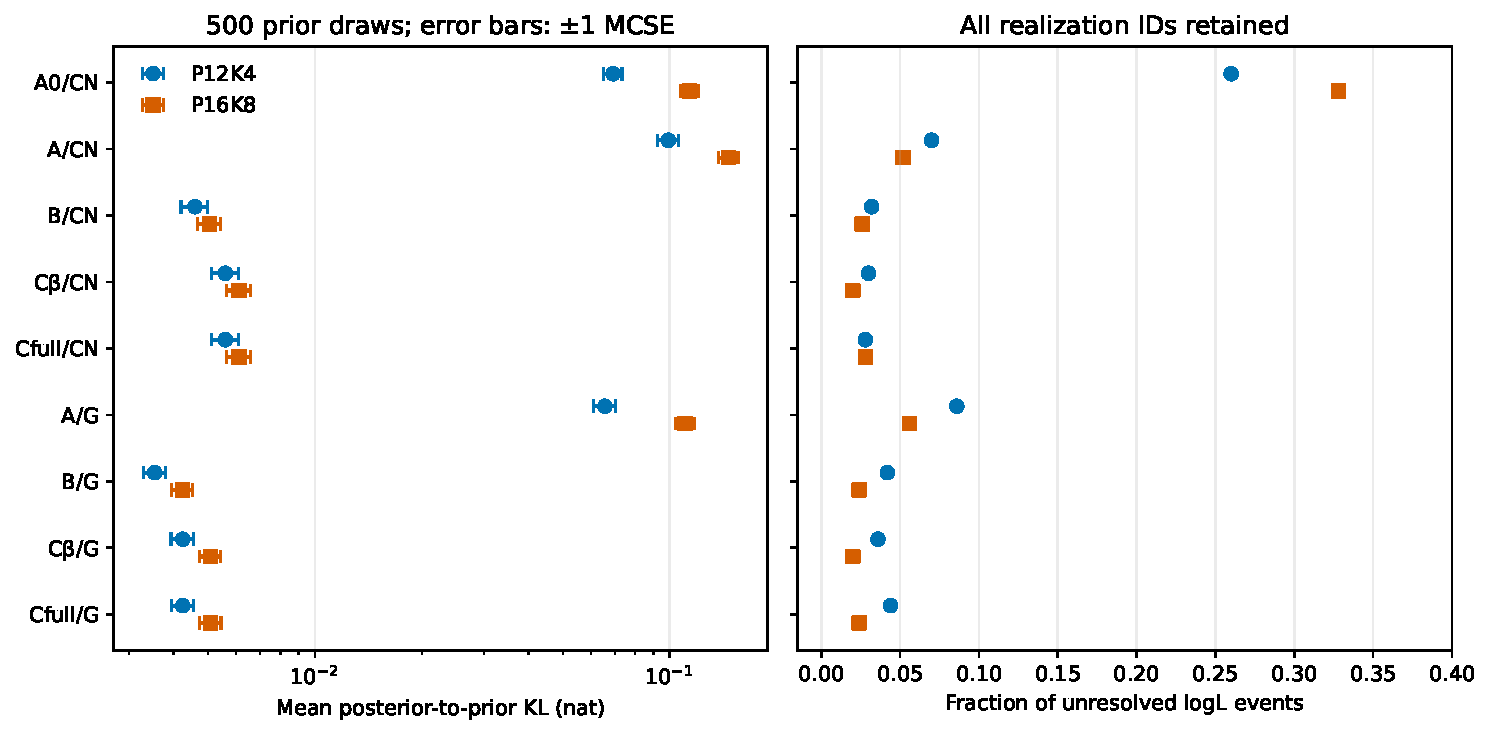
\includegraphics[width=\textwidth]{figures/information.pdf}
\caption{Prior-only information and numerical resolution in the completed campaign. Left: mean posterior-to-prior KL divergence, with one Monte Carlo standard error. Right: fraction of unresolved log-likelihood events among 500 prior draws. P12K4 and P16K8 are shown separately. Under approximate models, KL is descriptive rather than mutual information of the true generator.}
\end{figure}

For the correctly specified Gaussian control, the paired A/G minus B/G mean KL is $0.06211\pm0.00477$ nat in P12K4 and $0.10631\pm0.00695$ nat in P16K8. Because B is a fixed compression of A, the prior-average difference estimates information loss. The reported uncertainty reflects simulation variation, not systematic numerical error. Individual realizations need not exhibit this ordering. For a correctly specified model and deterministic $B=W A$, the identity
\begin{equation}
 \mathbb E_A D_{\rm KL}[p(u\mid A)\Vert p(u)]-
 \mathbb E_B D_{\rm KL}[p(u\mid B)\Vert p(u)]
 =I(u;A\mid B)\geq0
\end{equation}
follows from the chain rule of mutual information. Equality requires conditional sufficiency, $u\perp A\mid B$. This identity does not apply to approximate posterior families as though they were generated by the true joint distribution.

Compressed posteriors are weakly informative in this design. Similarity between B and frozen-response controls therefore does not validate the latter across other distances, spectra or signal strengths. Nor can this experiment separate the effect of increasing pulsar count from increasing frequency coverage. Raw complex data are nested, whereas the two sets of angular summaries need not be nested.

The fixed cells provide conditional recovery rather than SBC. At $u=0$, a central credible interval under a continuous prior structurally excludes the boundary; zero central coverage is not a numerical failure. Count intervals and binomial uncertainty are retained in the machine-readable results, rather than removing difficult realizations.

\section{Discussion and limits}
The principal evidence is a controlled separation: compression loses information in an exactly Gaussian experiment, while a normal approximation to physical quadratic estimators can fail calibration. These are distinct findings. They do not show that every effective-frequency response is biased, nor do they establish universal equivalence of B and C. Earlier matched response comparisons in the companion programme remained inconclusive at their predefined equivalence scale after numerical uncertainty was propagated.

The broader dissertation also reconstructs the historical linear massive-wave calculation and extends the experiment to linked Fierz--Pauli helicity zero. Transverse and longitudinal scalar deformations there belong to one degree of freedom and require cross terms in the response. The scalar population amplitude is phenomenological. Conditional recovery and local Fisher diagnostics do not constitute a fully marginalized observational inference or a detection claim. Those results provide context and complementary validation rather than additional samples of the present SBC experiment.

Real timing observations require an irregular sampling and timing-model adapter, stochastic-noise configuration and a reproduced public benchmark. A complex transformation of real residuals can introduce nonzero pseudocovariance and cross-frequency dependence. The availability of public TOAs does not justify applying the periodic likelihood unchanged. Only the sky directions in this campaign are observational metadata.

The work supports a methodological manuscript for review. Its limitations include known nuisance parameters, finite numerical validation, limited learning in compressed scenarios and unresolved likelihood events. No observational mass bound is reported. Before institutional or journal submission, authorship, affiliation and the final independent reproduction must be settled.

\section*{Data and code availability}
Sources, configurations, numerical summaries, validation receipts and the cumulative dissertation are available at \url{https://github.com/flavioluiz/TGdoWayne}. The completed campaign is fixed by tag v0.11.0. The repository contains eight new C11 archives and two reused historical archives, with SHA-256 manifests and a restoration script covering 106941 logical files. Public sky metadata originate from MeerKAT, DOI \href{https://doi.org/10.57891/j0vh-5g31}{10.57891/j0vh-5g31}, under CC BY 4.0. Literature PDFs are downloaded locally through the catalog and are not indiscriminately redistributed.

Archive restoration and component tests have been verified in a separate directory. Historical cache indices preserve some absolute paths; byte restoration alone is not a claim of a complete relocated physical rerun. The final reproduction audit is tracked separately. No submission or acceptance has occurred.
\printbibliography
\end{document}
